\documentclass{article}
\usepackage[left=25mm,top=1in,bottom=0.5in]{geometry}
\usepackage{fancyhdr}
\usepackage{extramarks}
\usepackage{amsmath}
\usepackage{amsthm}
\usepackage{amsfonts}
\usepackage{tikz}
\usepackage[plain]{algorithm}
\usepackage{algpseudocode}
\usepackage{listings}
\usepackage{minted}
\usepackage{graphicx}
\usepackage[dvipsnames]{xcolor}
\graphicspath{ {./} }
\definecolor{codegreen}{rgb}{0,0.6,0}
\definecolor{codegray}{rgb}{0.5,0.5,0.5}
\definecolor{codepurple}{rgb}{0.58,0,0.82}
\definecolor{backcolour}{rgb}{0.95,0.95,0.92}

\lstdefinestyle{mystyle}{
    backgroundcolor=\color{backcolour},
    commentstyle=\color{codegreen},
    keywordstyle=\color{magenta},
    numberstyle=\tiny\color{codegray},
    stringstyle=\color{codepurple},
    basicstyle=\ttfamily\footnotesize,
    breakatwhitespace=false,         
    breaklines=true,                 
    captionpos=b,                    
    keepspaces=true,                 
    numbers=left,                    
    numbersep=5pt,                  
    showspaces=false,                
    showstringspaces=false,
    showtabs=false,                  
    tabsize=2
}
\pagestyle{fancy}
\lhead{DEEKSHA ARORA}
\chead{CS 685}
%\rhead{\firstxmark}
\lfoot{\lastxmark}
\cfoot{\thepage}

\title{CS 685 (Data Mining)
Assignment 1}
\author{\textbf{DEEKSHA ARORA} \\ Roll No. 20111017}
\date{Due date: September 25, 2020 \\ Instructor: Prof. Arnab Bhattacharya}

\newcommand{\enterProblemHeader}[1]{
    \nobreak\extramarks{}{Problem \arabic{#1} continued on next page\ldots}\nobreak{}
    \nobreak\extramarks{Problem \arabic{#1} (continued)}{Problem \arabic{#1} continued on next page\ldots}\nobreak{}
}

\newcommand{\exitProblemHeader}[1]{
    \nobreak\extramarks{Problem \arabic{#1} (continued)}{Problem \arabic{#1} continued on next page\ldots}\nobreak{}
    \stepcounter{#1}
    \nobreak\extramarks{Problem \arabic{#1}}{}\nobreak{}
}

\setcounter{secnumdepth}{0}
\newcounter{partCounter}
\newcounter{homeworkProblemCounter}
\setcounter{homeworkProblemCounter}{1}
\nobreak\extramarks{Problem \arabic{homeworkProblemCounter}}{}\nobreak{}

\newenvironment{homeworkProblem}[1][-1]{
    \ifnum#1>0
        \setcounter{homeworkProblemCounter}{#1}
    \fi
    \section{Problem \arabic{homeworkProblemCounter}}
    \setcounter{partCounter}{1}
    \enterProblemHeader{homeworkProblemCounter}
}{
    \exitProblemHeader{homeworkProblemCounter}
}

\begin{document}

\maketitle
\pagebreak
\lstset{style=mystyle}
\begin{center}
\section{{REPORT}}
\end{center}
\subsection{ANALYSIS}
Some key questions which prevail among all individuals today are how the disease, COVID-19 would propagate in an environment in which it is left unconstrained? or whether the initial lockdown was successful? In the present study, the drilldown analysis of Covid-19 cases in India is presented and also discusses the effect of COVID-19 on population of the country.\\
In the second week of March, WHO declared the Novel Coronavirus Disease (COVID-19) outbreak as a pandemic (an epidemic that has spread worldwide affecting a large number of people).  In India, on 14th March there were a total of 84 cases reported in Delhi, Karnataka, Kerala, Maharashtra and Uttar Pradesh. At this time the government imposed the first lockdown in order to stop the spread of the Novel Coronavirus disease. Even after country-wide lockdown the number of cases kept on increasing in India. By the end of March, the states with most cases were Maharashtra, Kerala, Delhi, Uttar Pradesh and Rajasthan while the number of cases in other states were much less as compared to these 5 states. 
In the month of April, Mumbai, Chennai, Ranchi, Ahmedabad and Indore were the hotspot districts in their states. In May, approximately ten thousand cases were reported daily and the top five hotspot cities were Puducherry, Chennai, Ahmedabad, Mumbai and Changlang. By the end of May, the increase in number of cases was ten times more than the increase in the month of April. In June, the daily rise of cases was approximately ten thousand and the hotspot districts were Chennai, Puducherry, Ahmedabad, Bengaluru and Gautam Buddha Nagar. In July, the daily count of positive cases increased to thirty thousand with a total of around 4 lakh positive cases by the end of July. The hotspot districts in the month of July were Bengaluru, Puducherry, Raipur and Aizawal. In August, the daily count of COVID-19 positive cases increased to sixty thousand with Puducherry, districts of west Tripura, Bengaluru, Aizawal and Raipur as the top hotspot districts. The top five hotspot districts for the duration 15 March 2020 to 5 Sept 2020 are Bengaluru, Chennai, Puducherry, Raipur and Patna.\\
The weekly analysis of data shows that Delhi was the hotspot district in its region in initial weeks. In Delhi, the number of positive cases were 20 and 22 in week 1(15 -21 March 2020) and week 2 (22-28 March 2020) but in week 3 the number of cases sparked to 396, following which the cases nearly doubled every week, till mid- July. In the later half of July, there was a constant increase in COVID-19 positive cases in Delhi and this trend followed till end of August. In Mumbai, the number of cases spiked in the the month of May and since then the cases have been increasing every week going as far as ten thousand positive cases in one week.\\
\begin{figure}[h]
\centerline{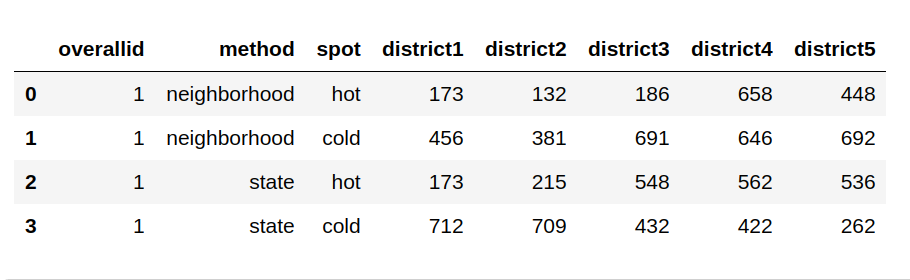
\includegraphics[scale=0.5]{photo1.png}}
\caption{Hotspot and Coldspot Districts using overall analysis }
\label{fig}
\end{figure}
The overall trend shows Bengaluru urban region (district id =173) as the top hotspot district. Bengaluru had zero cases till mid-June. After that the cases in Bengaluru urban region had a steady growth and till 5 Sept, 2020 the number of cases in  Bengaluru surpassed Delhi and other hotspot districts in the initial weeks. Bhopal(district id=186) is hotspot district in its neighborhood but it is not a hotspot district in it's state because the cases in Bhopal are less as compared to other districts in Madhya Pradesh.
The overall analysis shows that the top hotspot district in its state is Bengaluru urban region and after that Chennai(distrcit id=215) is the second top hotspot district. In Chennai, the positive cases in week 7 were 732 following which there was a sudden spike in cases in week 8 with 2065 cases. After that there was a steady rise in cases till end of June following which the number of cases had a steady decline upto 5 Sept, 2020. The third top hotspot district is Puducherry (district id =548). The positive cases in Puducherry started increasing in mid-May and since then the cases have steadily increased.\\
The overall trend of analysis also shows that Wayanad (district id= 712) is the top coldspot district in it's state(Kerala). The number of positive cases in Wayanad district in last week of August were 206, very less s compared to other districts of Kerala.

\subsection{EFFECT ON POPULATION}
Along with its high infectivity and fatality rates, the 2019 Corona Virus Disease (COVID-19) has caused universal psychosocial impact by causing mass hysteria, economic burden and financial losses.  Disease itself multiplied by forced quarantine to combat COVID-19 applied by nationwide lockdowns has produced acute panic, anxiety, obsessive behaviors, hoarding, paranoia, and depression, and post-traumatic stress disorder (PTSD) in the long run.
\subsection{EFFECT ON CHILDREN }
Community-based mitigation programs to combat COVID-19 has disrupted children’s usual lifestyle and has caused florid mental distress. These effects are expected to be the most damaging for children in the poorest countries, and in the poorest neighborhoods and for those in already disadvantaged or vulnerable situations. Children have been experiencing worry, anxiety and fear,  such as the fear of dying, the fear of losing one's relatives, or the fear of what it means to receive medical treatment. This is a universal crisis and for some children, the impact will be lifelong.
\subsection{EFFECT ON OLDER PEOPLE}
The psychosocial aspects of older people are affected by this pandemic in different ways and need special attention.COVID-19 has changed older people’s daily routines, the care and support they receive and their ability to stay socially connected. Older people are being challenged by requirements to spend more time at home, lack of physical contact with other family members, friends and colleagues  and anxiety and fear of illness and death – their own and others. Some older people who were already socially isolated have experienced loneliness which has resulted in worse mental health.
\subsection{EFFECT ON HEALTHCARE WORKERS}
In the developing countries like India, where the health care system is already overburdened, surges of COVID-cases has provoked acute anxiety, irritation and stress among doctors and nurses. This might be compounded by the inadequate hospital supply of required hand hygiene tools and significant shortage of personal protective equipment (PPE) among HCPs, who are at the highest risk of transmission.
\section{CONCLUSION}
With each passing day more and more number of people are affected by the spread by Novel Coronavirus. Despite various measures like implementation of country -wide lockdown, increase in capacity of quarantine centers, improvement in testing facilities, etc the spread has not stopped, infact the situation became more and more serious with each passing day. It is extremely difficult to predict when will the spread of coronavirus will stop.\\
The enforced shift during the worst of the pandemic to virtual working, has affected ways of communicating across learning, working and transacting. This has resulted in adoption of digital by those who were yet to do so. Winners are those who have tested and explored all of the associated creative possibilities in this pandemic. 
\end{document}
